% !TeX program = pdflatex
% IJCV submission version. Springer Nature template (sn-jnl.cls), author-year references.
% Files needed in the same folder: sn-jnl.cls, sn-mathphys-ay.bst, references.bib and all figure files.
\documentclass[pdflatex,sn-mathphys-ay]{sn-jnl}

\usepackage{graphicx}
\usepackage{multirow}
\usepackage{amsmath,amssymb,amsfonts}
\usepackage{xcolor}
\usepackage{textcomp}
\usepackage{booktabs}
\usepackage{array,tabularx}
\usepackage{colortbl}
\usepackage{placeins}
\usepackage{url}

\definecolor{SeaBlue}{HTML}{5878A6}
\definecolor{SoftBlue}{HTML}{A7C7E7}
\definecolor{Coral}{HTML}{F4A7AE}
\definecolor{SeaTeal}{HTML}{A6D0C6}
\newcommand{\heatcell}[2]{\cellcolor[HTML]{#1}#2}
\newcolumntype{Y}{>{\raggedright\arraybackslash}X}

\newcommand{\codeurl}{\url{https://github.com/Fuyulin-hub/vlm-guided-3d-parts}}

% Fix: \burl fallback in the .bbl is \textsf, which breaks URLs containing underscores.
\providecommand{\burl}[1]{\url{#1}}

\raggedbottom

\begin{document}

\title[Decoupling Mask Refinement and Assembly for 3D Part Segmentation]{Decoupling Mask Refinement and Assembly for 3D Part Segmentation}

\author[1]{\fnm{Yulin} \sur{Fu}}\email{fyulin2024@lzu.edu.cn}

\author[1]{\fnm{Cheng} \sur{Yang}}\email{ycheng2026@lzu.edu.cn}
\equalcont{These authors contributed equally as second authors.}

\author[1]{\fnm{Qing} \sur{Ai}}\email{aiq2026@lzu.sysu.edu.cn}
\equalcont{These authors contributed equally as second authors.}

\author*[1]{\fnm{Jisheng} \sur{Dang}}\email{dangjisheng@lzu.edu.cn}

\author*[2]{\fnm{Bin} \sur{Hu}}\email{bh@bit.edu.cn}

\author[3]{\fnm{Wei-Shi} \sur{Zheng}}\email{wszheng@outlook.com}

\author[4]{\fnm{Qi} \sur{Tian}}\email{wywqtian@gmail.com}

\author[5]{\fnm{Tat-Seng} \sur{Chua}}\email{dcscts@nus.edu.sg}

\author[6]{\fnm{Qibin} \sur{Hu}}

\affil[1]{\orgname{Lanzhou University}, \orgaddress{\city{Lanzhou}, \country{China}}}

\affil[2]{\orgname{Beijing Institute of Technology}, \orgaddress{\city{Beijing}, \country{China}}}

\affil[3]{\orgdiv{School of Computer Science and Engineering}, \orgname{Sun Yat-sen University}, \orgaddress{\city{Guangzhou}, \country{China}}}

\affil[4]{\orgname{Huawei Consumer Business Group}, \orgaddress{\city{Shenzhen}, \country{China}}}

\affil[5]{\orgdiv{School of Computing}, \orgname{National University of Singapore}, \orgaddress{\country{Singapore}}}

\affil[6]{\orgname{Sun Yat-sen University}, \orgaddress{\city{Shenzhen}, \country{China}}}

\abstract{Guiding 3D part segmentation requires resolving overlaps between independently predicted part masks. When revised prompts also set assembly priorities, correcting a mask changes both its prediction and its arbitration against other masks. We separate these operations using original spatial anchors. A vision-language model (VLM) audit revises the Segment Anything Model 2 (SAM2) predictions, while the initial points and boxes govern component selection and assembly priority. With masks fixed, retry-box ordering changes pixel ownership on 75 of 471 objects. Compared with raw-image SegviGen, our guidance improves the projected mean intersection over union (mIoU) and the five-pixel boundary F1 (BF1) by an absolute 4.14\% and 4.39\%, respectively. On 14 paired PartObjaverse-Tiny meshes, it improves instance intersection over union (IoU) over raw-image guidance, while automatic SAM2 guidance leads on both native metrics. Our code is available at \codeurl.}

\keywords{3D part segmentation, vision-language models, spatial anchors, mask refinement}

\maketitle

\section{Introduction}\label{sec:introduction}

Local editing of assets generated by Zero-1-to-3 \citep{liu2023zero123} or TRELLIS.2 \citep{xiang2025trellis2} requires explicit parts. Components such as a grille and a housing can share appearance despite their different functions, so separating them requires both semantic intent and spatial evidence. Recent work addresses this need from several directions. PartCrafter \citep{lin2025partcrafter} and PartGen \citep{chen2024partgen} generate parts directly. Find3D \citep{ma2024find3d} uses queries, PartField \citep{liu2025partfield} uses features, and P3-SAM \citep{ma2025p3sam} and PartSAM \citep{zhu2025partsam} predict 3D masks. SA3D \citep{cen2025sa3d} and GeoSAM2 \citep{deng2025geosam2} instead propagate image masks to 3D. SegviGen \citep{li2026segvigen} accepts a source-view part map, which exposes a guidance interface between image interpretation and 3D segmentation.

Automatic masks from Mask2Former \citep{cheng2022mask2former} and the Segment Anything Model (SAM) \citep{kirillov2023sam} can merge functional parts, as the grille and the service panel in Fig.~\ref{fig:motivation} show, while independently prompted masks can overlap or leave gaps. An assembly step must therefore assign each foreground pixel to exactly one part. A prompt box can both localize a mask and set its assembly priority. For example, enlarging a grille box beyond a competing housing box gives the housing priority even when both masks are fixed. Prompt metadata thus couples the correction of a prediction to the arbitration of overlaps.

\begin{figure}[t]
\centering
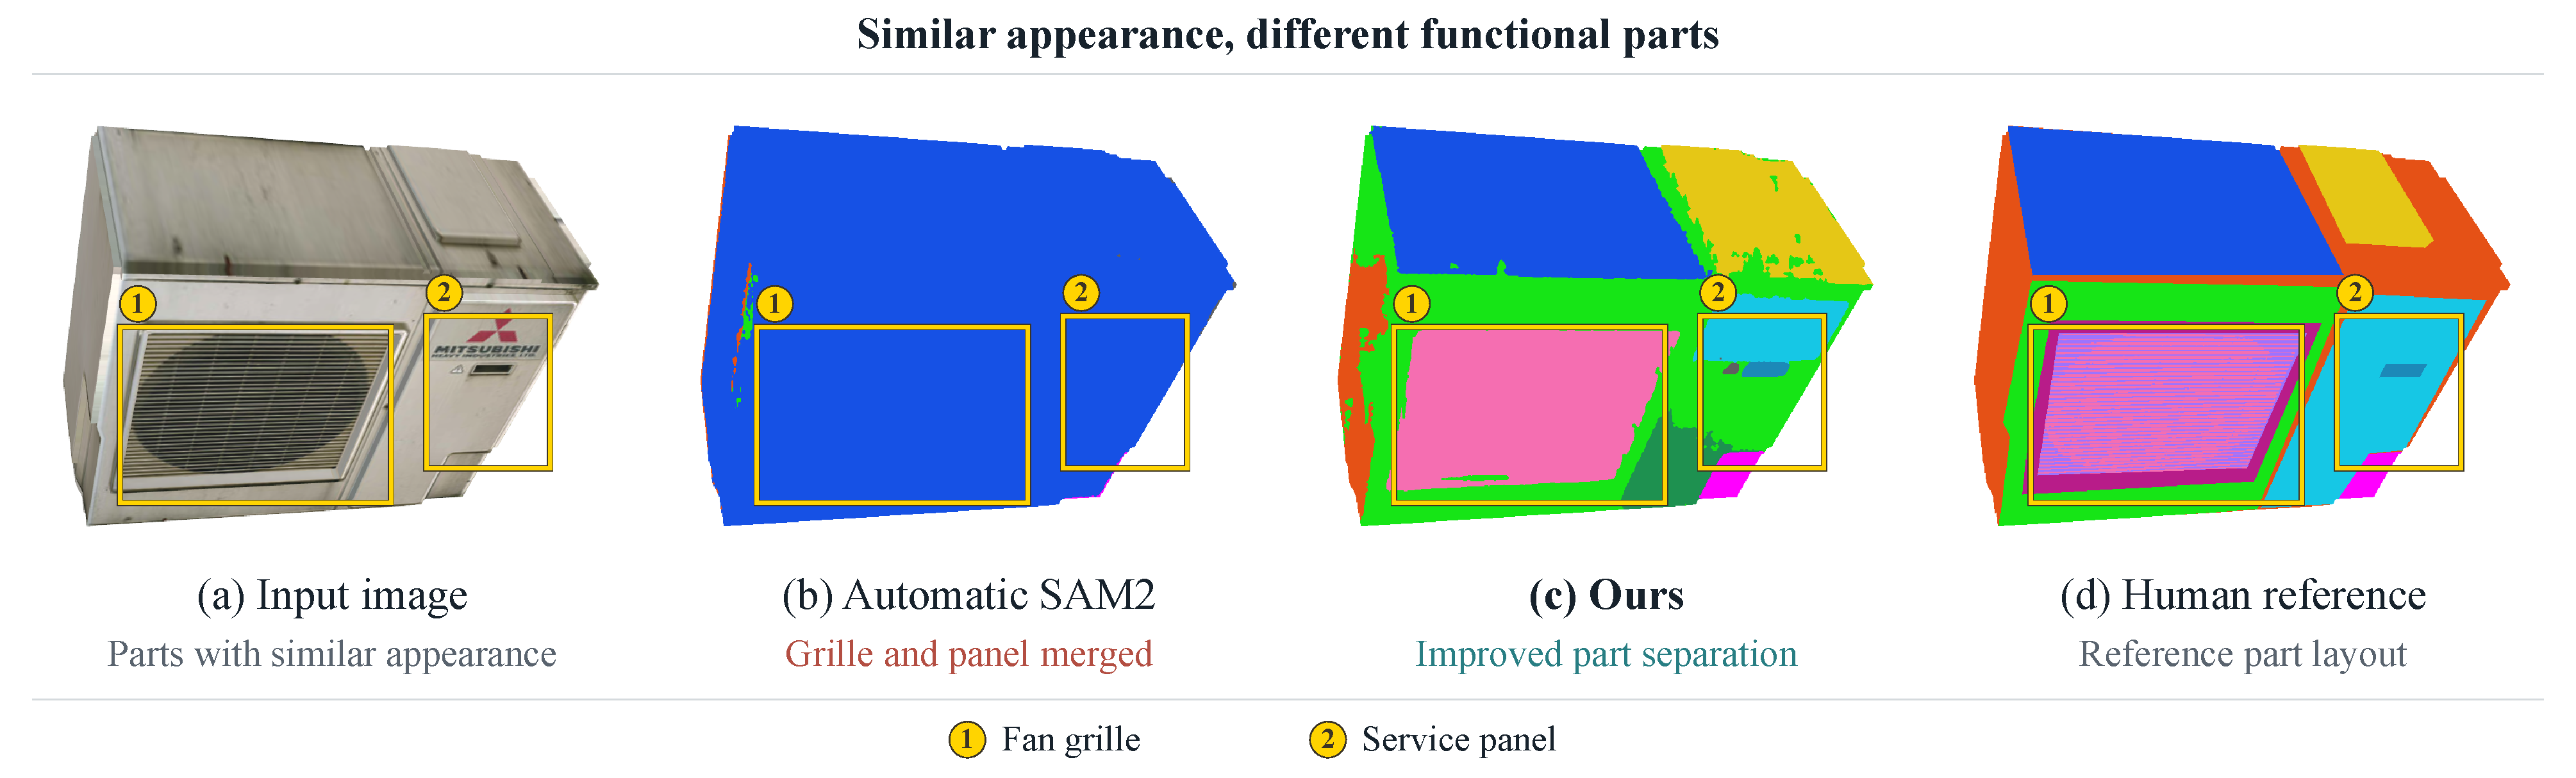
\includegraphics[width=\textwidth]{fig1_motivation.pdf}
\caption{Source image, automatic guidance, Ours, and reference. Yellow boxes mark the grille and service panel, and display colors are matched without changing boundaries.}
\label{fig:motivation}
\end{figure}

We retain separate spatial references for prediction and assembly. Qwen3-VL \citep{bai2025qwen3vl} plans visible parts with boxes and points, and SAM2 \citep{ravi2024sam2} predicts their masks. A single audit can revise the prediction prompts and replace a mask. Assembly instead uses the original positive point to select a component and the original box area to set its primary priority. Updated masks remain free to change the pixels they claim, so the separation fixes which prompt metadata governs assembly without freezing the partition itself.

The contributions of this work are threefold. First, we define an explicit interface that separates revisable prediction prompts from the original spatial anchors used for assembly. Second, we design controls that distinguish the effects of the two operations, including box substitution with fixed masks and ablations of mask selection, filtering, and ordering with a frozen SegviGen. Third, we evaluate source-view agreement, output projections on 471 objects, and official annotations on disjoint meshes, and the results distinguish boundary agreement from part recovery.

\section{Related Work}\label{sec:related}

\subsection{3D Part Representations}
PointNet \citep{qi2017pointnet} learns point features, while PartNet \citep{mo2019partnet} and latent part-whole models \citep{gao2025latent} address hierarchy. \citet{umam2024copart} aggregate superpoints for unsupervised co-part segmentation. PartSLIP \citep{liu2023partslip} and PartDistill \citep{umam2024partdistill} transfer image-language knowledge, and LASO \citep{li2024laso} predicts language-specified affordances. Find3D \citep{ma2024find3d} uses queries, PartField \citep{liu2025partfield} clusters features, and P3-SAM \citep{ma2025p3sam} and PartSAM \citep{zhu2025partsam} predict 3D masks. Our focus is assembling 2D candidates into a conditioning partition.

\subsection{Language and Spatial Prompts}
CLIP \citep{radford2021clip} aligns image-text features, Grounding DINO \citep{liu2024groundingdino} localizes objects, and DenseCLIP \citep{rao2022denseclip} and OpenSeeD \citep{zhang2023openseed} enable dense prediction. EARN \citep{liu2023earn} and ReferDINO \citep{liang2025referdino} address expression grounding and video segmentation, respectively. DM-PCL \citep{han2025dmpcl} and GMENet \citep{michieli2022gmenet} model part supervision and spatial relations, respectively. We use promptable segmentation models such as SAM \citep{kirillov2023sam} and SAM2 \citep{ravi2024sam2}, with revisable prediction prompts and fixed assembly anchors.

\subsection{Propagation of 2D Evidence}
LERF \citep{kerr2023lerf} transfers features to radiance fields, while Feature 3DGS \citep{zhou2024feature3dgs} and Semantic Gaussians \citep{guo2026semanticgaussians} transfer them to 3D Gaussians \citep{kerbl20233dgs}. OpenScene \citep{peng2023openscene} and PLA \citep{ding2023pla} align 3D and image-language features. OmniSeg3D \citep{ying2024omniseg3d} learns hierarchy, whereas SAI3D \citep{yin2024sai3d} and Open3DIS \citep{nguyen2024open3dis} aggregate multiview masks. Memory sampling \citep{dang2023efficient}, scene-motion-instance decomposition \citep{dang2026videodecoupling}, and SAM2Object \citep{zhao2025sam2object} exploit temporal evidence. GeoStyler \citep{hu2026geostyler} preserves geometry during style transfer. SA3D \citep{cen2025sa3d} and GeoSAM2 \citep{deng2025geosam2} propagate masks. We follow the controlled analysis of \citet{yang2024benchmark} to examine guidance construction with SegviGen frozen \citep{li2026segvigen}.

\section{Method}\label{sec:method}

\subsection{Refinement and Assembly Interface}
Given a red-green-blue-alpha (RGBA) rendering $I$, let $I_{\mathrm{rgb}}$ denote its color channels and $F_\alpha=\{x\mid\alpha(x)>10\}$ its foreground. Assembly takes selected masks $\widehat M_i$, initial boxes $b_i$, and initial positive points $p_i$ as
\begin{equation}
L=\mathcal A\bigl(\{(\widehat M_i,b_i,p_i)\}_i,F_\alpha\bigr).
\label{eq:assembly_interface}
\end{equation}
Revised prompts affect $\mathcal A$ through selected masks. With masks and initial anchors fixed, changing retry metadata leaves $L$ unchanged. Mask updates can still alter connectivity, overlaps, and mask-area tie breaks. We encode $L$ as guidance $G$ for frozen SegviGen with a shared voxel asset $V$, as illustrated in Fig.~\ref{fig:pipeline}.

\begin{figure}[t]
\centering
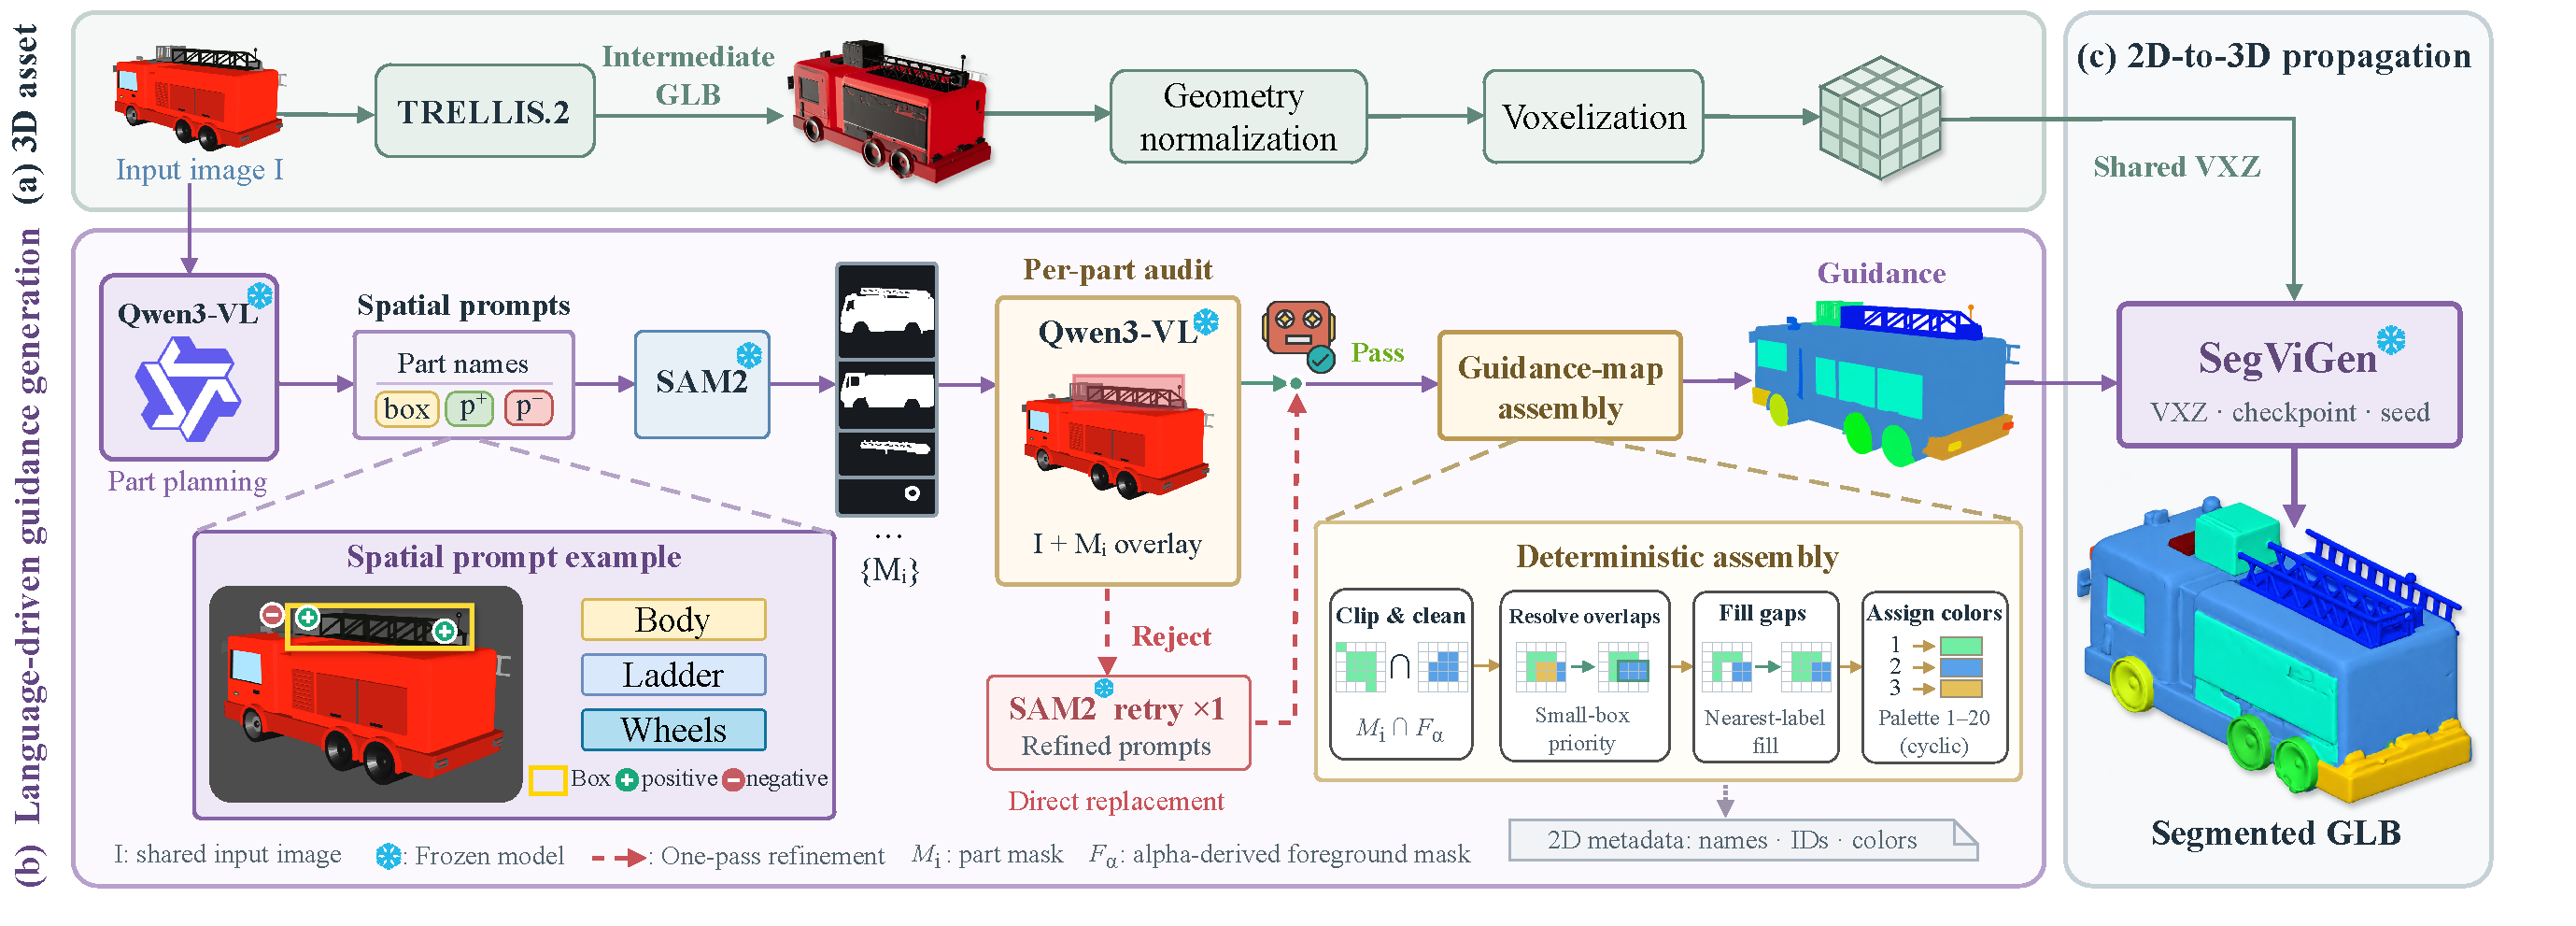
\includegraphics[trim=5.0bp 18.9bp 42.1bp 5.0bp,clip,width=\textwidth]{fig2_pipeline.pdf}
\caption{Language-guided 3D segmentation with shared geometry. The audit revises prediction prompts, while assembly retains the original anchors. Names and identifiers (IDs) are 2D metadata, and they do not affect assembly.}
\label{fig:pipeline}
\end{figure}

TRELLIS.2 \citep{xiang2025trellis2} reconstructs a GL Transmission Format Binary (GLB) mesh for fixed normalization, coordinate conversion, and VXZ voxelization. This mesh can differ from the source. The four compared conditions, namely A (raw-image guidance), B (automatic SAM2 guidance), C (our guidance), and D (reference guidance), share the reconstructed geometry, checkpoint, settings, and seed, with source orientation, preprocessing, and camera identity recorded.

\subsection{Visible Part Planning and Spatial Prompts}
Qwen3-VL proposes $r_i=(n_i,b_i,P_i^+,P_i^-)$, comprising a visible part name, a box, and positive and negative points \citep{bai2025qwen3vl}. Repeated parts retain distinct prompts. Coordinates in $[0,1000]$ are converted to pixels and clipped. After foreground adjustment, the first valid positive point $p_i$ and the initial box $b_i$ become fixed assembly anchors. Unsupported proposals are logged and skipped.

Frozen SAM2 predicts $M_i^{(0)}=S_\theta(I_{\mathrm{rgb}},b_i,P_i^+,P_i^-)$ using all valid points and disabling multimask prediction. Names remain metadata, and predicted quality is stored separately from reference scores.

\subsection{Mask Refinement Through One-Pass Audit}
Interactive refinement uses clicks \citep{jain2019click}, feature optimization \citep{sofiiuk2020fbrs}, prior masks \citep{sofiiuk2022ritm}, local corrections \citep{chen2022focalclick}, and transformers \citep{liu2023simpleclick}. Our VLM audits the source image, the target name, and a red mask overlay with a two-pixel contour, as shown in Fig.~\ref{fig:audit_assembly}a. Accepted candidates retain $M_i^{(0)}$, whereas a rejection permits an updated box and additional points, followed by one SAM2 retry as
\begin{equation}
M_i^{(1)}=S_\theta(I_{\mathrm{rgb}},\widetilde b_i,
P_i^+\cup\Delta P_i^+,P_i^-\cup\Delta P_i^-).
\label{eq:refinement}
\end{equation}

\begin{figure}[t]
\centering
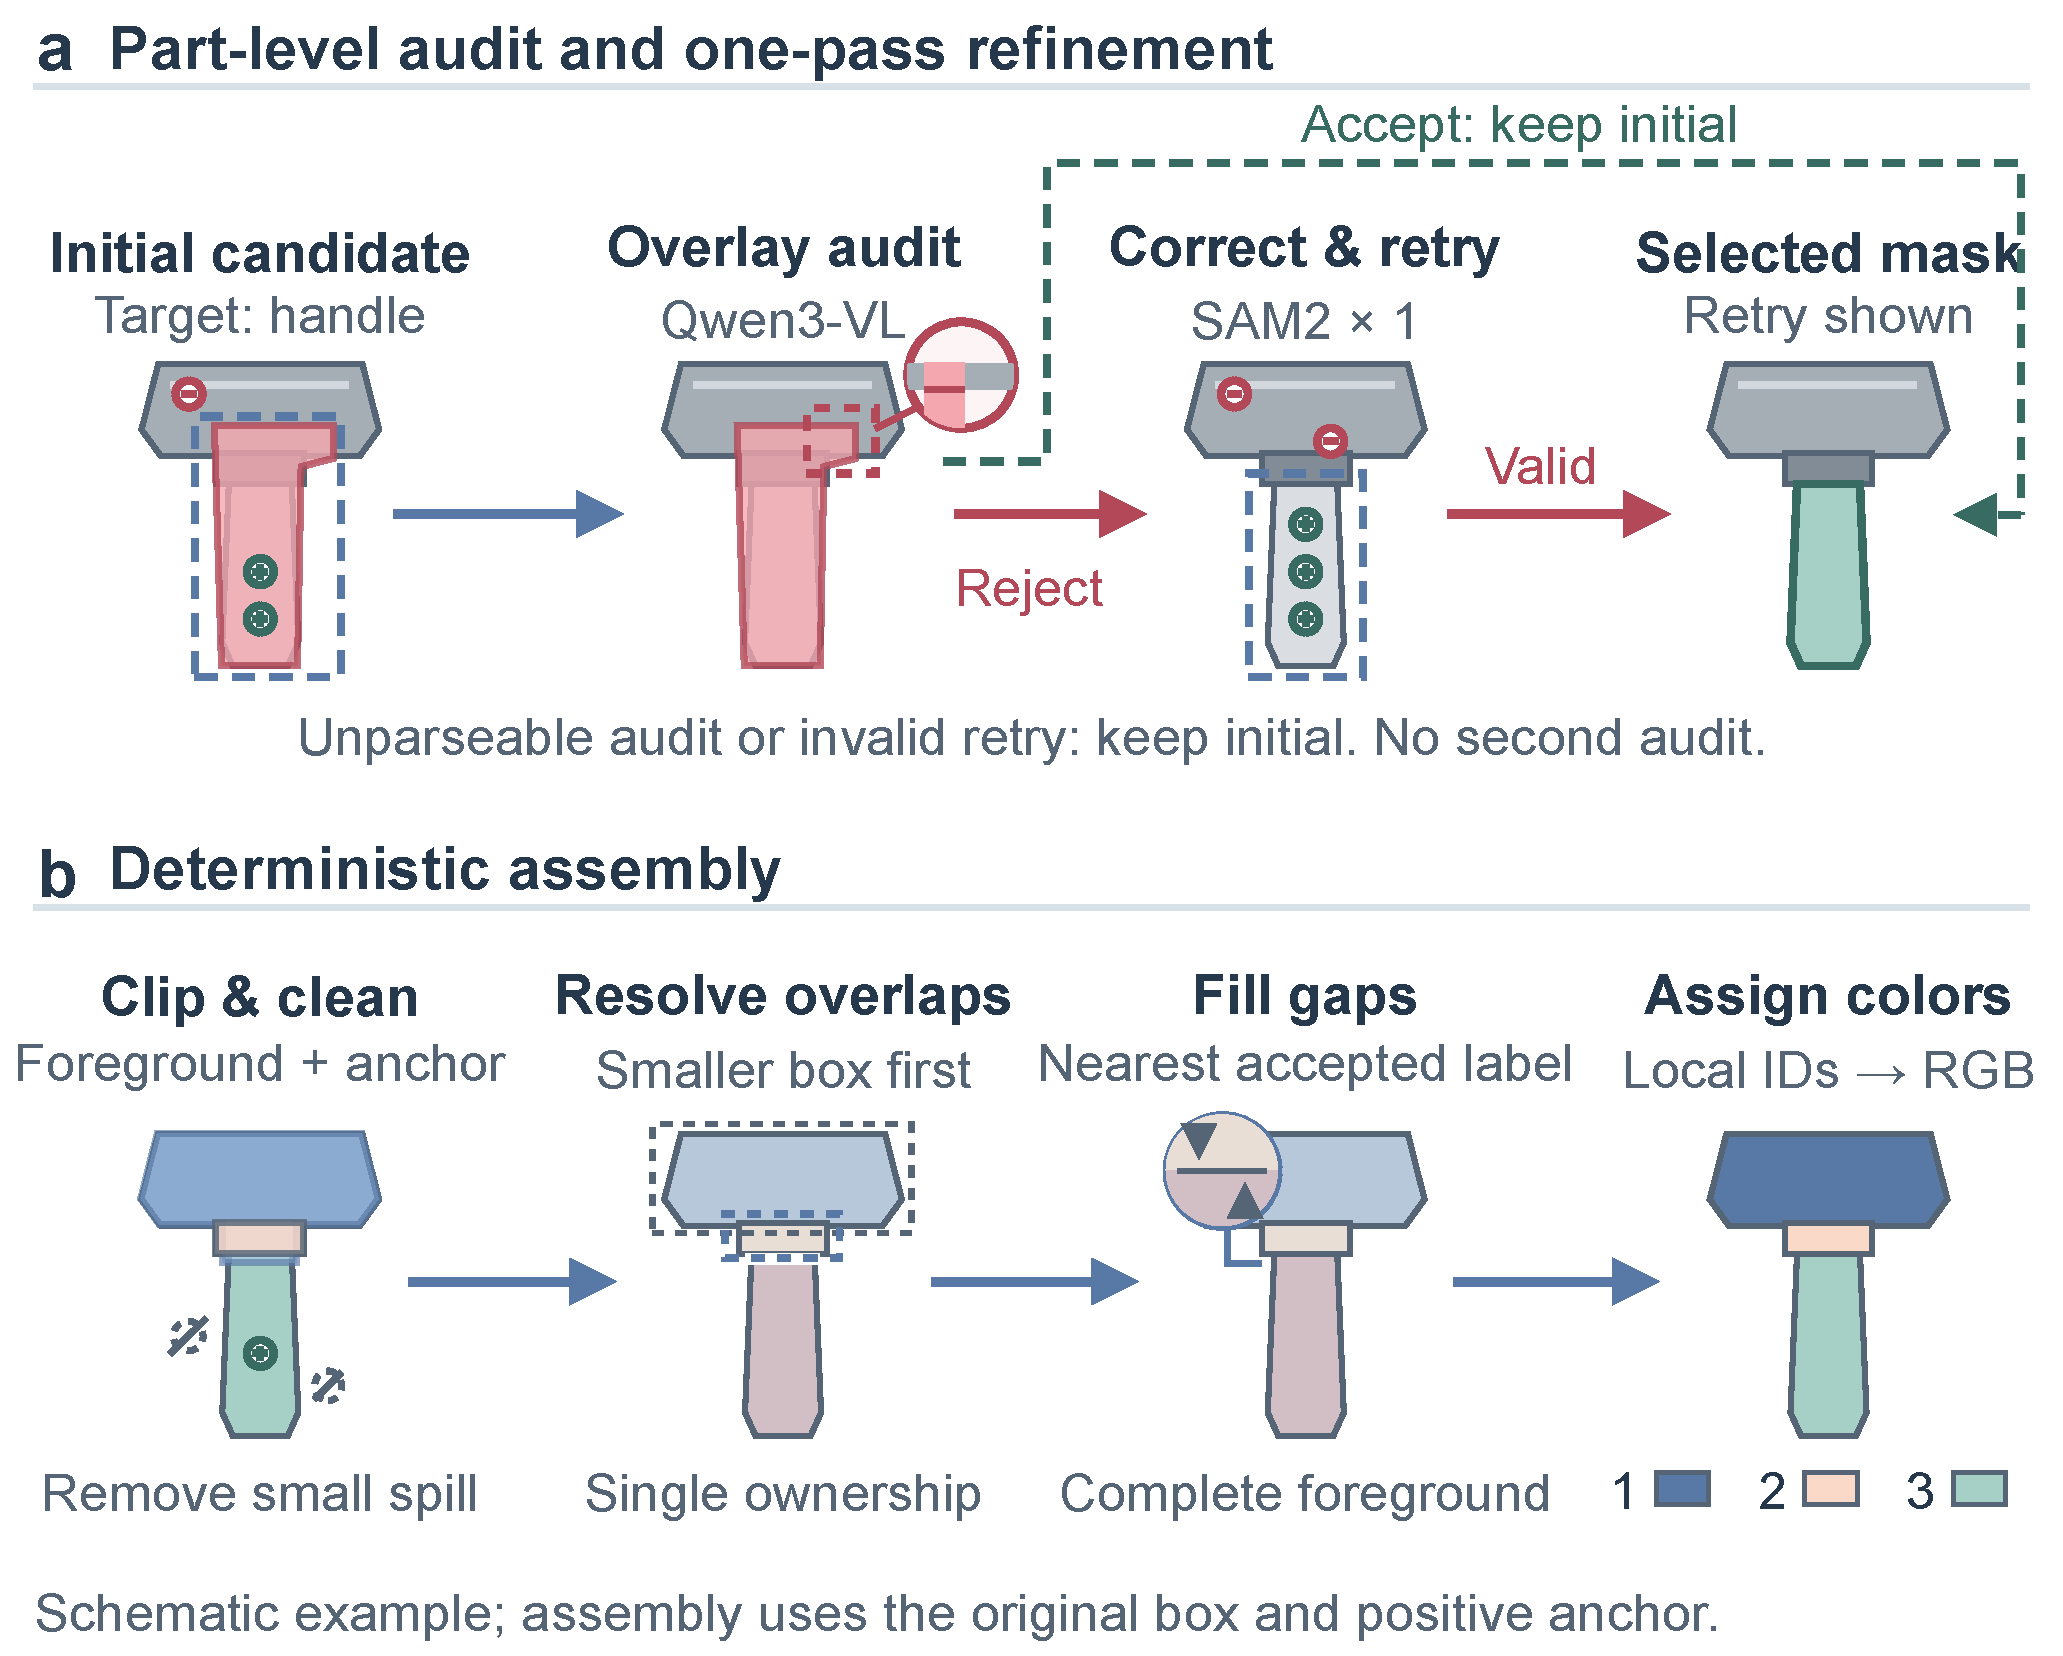
\includegraphics[width=0.95\textwidth]{fig_audit_assembly_single_column.pdf}
\caption{Separate controls for refinement and assembly. \textbf{a}, One prompt correction can replace a mask. Invalid audit or retry retains it. \textbf{b}, Original points select connected components, and original boxes set the primary overlap priority of each part.}
\label{fig:audit_assembly}
\end{figure}

A valid retry becomes the selected mask $\widehat M_i$ without further audit or overlap-based selection. Otherwise $\widehat M_i=M_i^{(0)}$, with parsing and retry failures logged. The audit passes $\widehat M_i$ to assembly together with $(b_i,p_i)$ from the initial plan. For $N$ initial predictions and $K_v\leq N$ valid masks, there are $K_v$ audits and at most $K_v$ retries, which gives at most $2N$ SAM2 calls.

\subsection{Region Assignment from Original Anchors}

\subsubsection{Clip and Clean}
Cleaning clips $\widehat M_i$ to $F_\alpha$ and selects the eight-connected component containing the original $p_i$, or the nearest component if $p_i$ lies outside. The largest component is used without an anchor. Additional components require area $\geq\max(96,\lfloor0.18a_i\rfloor)$ for main-component area $a_i$. A $3\times3$ elliptical closing, foreground clipping, and a second filtering pass yield $\overline M_i$. Enclosed holes up to $\max(48,\lfloor0.00015|F_\alpha|\rfloor)$ pixels are filled, excluding boundary-connected background. Candidates require at least $\max(a_{\min},96,\lfloor0.00012|F_\alpha|\rfloor)$ pixels, with $a_{\min}=10$.

\subsubsection{Resolve Overlaps}
Candidates are sorted lexicographically by $(|b_i|,|\overline M_i|,\mathrm{ID}_i)$, where $|b_i|$ is the initial box area. Smaller boxes claim supported pixels first, and cleaned mask area and ID break ties. This rule treats the initial box extent as a localization prior. Each candidate contributes unoccupied pixels $R_{\pi(t)}=\overline M_{\pi(t)}\setminus U_{t-1}$ if at least $\max(a_{\min},96,\lfloor0.00010|F_\alpha|\rfloor)$ remain. Accepted regions enter $U$ and rejections are logged. The original point selects connected support, whereas the original box orders competing claims.

\subsubsection{Fill Gaps}
Each remaining foreground pixel inherits its nearest accepted label as
\begin{equation}
L(x)=L\!\left(\arg\min_{y\in U}\|x-y\|_2\right),
\quad x\in F_\alpha\setminus U.
\label{eq:gaps}
\end{equation}
A Euclidean distance transform preserves existing labels and background zero. If $U$ is empty, processing fails. Otherwise, the mutually exclusive regions cover $F_\alpha$.

\subsubsection{Assign Colors}
Accepted candidates receive sequential labels in assembly order. We save 16-bit labels before mapping background to $c_0$ and foreground $l$ to $c_{1+((l-1)\bmod20)}$. Reordering can therefore change colors even when candidate ownership is unchanged. Beyond 20 parts, red-green-blue (RGB) colors repeat but integer IDs remain distinct. Metadata retains names, IDs, palette indices, and masks.

\subsection{3D Propagation}
Frozen SegviGen predicts $\widehat{\mathcal G}_k=H_\phi(V,G_k;\xi)$ with weights $\phi$ and shared sampling settings $\xi$. The assembled partition enters through $G_k$, while names remain metadata. Output GLB regions are decoded for scoring.

\section{Experiments}\label{sec:experiments}

\begin{table}[t]
\caption{Projection agreement (\%). Five methods share 471 objects and object weighting, and shading is columnwise within this block. Find3D uses 468 objects, group weighting, and reference-assisted queries. Part F1 uses IoU 0.5.}
\label{tab:main}
\setlength{\tabcolsep}{3pt}
\begin{tabularx}{\textwidth}{@{}Y >{\raggedright\arraybackslash}p{1.9cm} c c c c c@{}}
\toprule
Method & Part condition & \shortstack{Proj. mIoU\\(\%) $\uparrow$} & \shortstack{BF1@5px\\(\%) $\uparrow$} & \shortstack{BF1@2px\\(\%) $\uparrow$} & \shortstack{Part F1@0.5\\(\%) $\uparrow$} & \shortstack{Evaluable\\$N$}\\
\midrule
PartField \citep{liu2025partfield} & Clustering & \heatcell{F3F8CD}{34.17} & \heatcell{FAEFCE}{25.80} & \heatcell{FAE3CF}{13.98} & \heatcell{FBD2D2}{17.46} & 471\\
P3-SAM \citep{ma2025p3sam} & Automatic & \heatcell{D1F5D0}{\textbf{40.05}} & \heatcell{E1F7CE}{32.67} & \heatcell{F3F8CD}{18.17} & \heatcell{D1F5D0}{\textbf{37.44}} & 471\\
GeoSAM2 \citep{deng2025geosam2} & Automatic views & \heatcell{FBD2D2}{26.08} & \heatcell{FBD2D2}{19.89} & \heatcell{FBD2D2}{11.40} & \heatcell{DDF6CF}{34.56} & 471\\
SegviGen \citep{li2026segvigen} & No part prompt & \heatcell{F4F8CD}{34.00} & \heatcell{E7F7CE}{31.48} & \heatcell{E4F7CE}{20.26} & \heatcell{E6F7CE}{32.27} & 471\\
Ours & 2D guidance & \heatcell{DCF6CF}{38.14} & \heatcell{D1F5D0}{\textbf{35.88}} & \heatcell{D1F5D0}{\textbf{23.07}} & \heatcell{D3F5D0}{36.84} & 471\\
\midrule
\multicolumn{7}{@{}l}{\textit{Separate reference-assisted setting, group-macro aggregation}}\\
Find3D \citep{ma2024find3d} & D-assisted queries & 30.66 & 30.66 & 26.38 & 33.03 & 468\\
\botrule
\end{tabularx}
\end{table}

\begin{figure}[t]
\centering
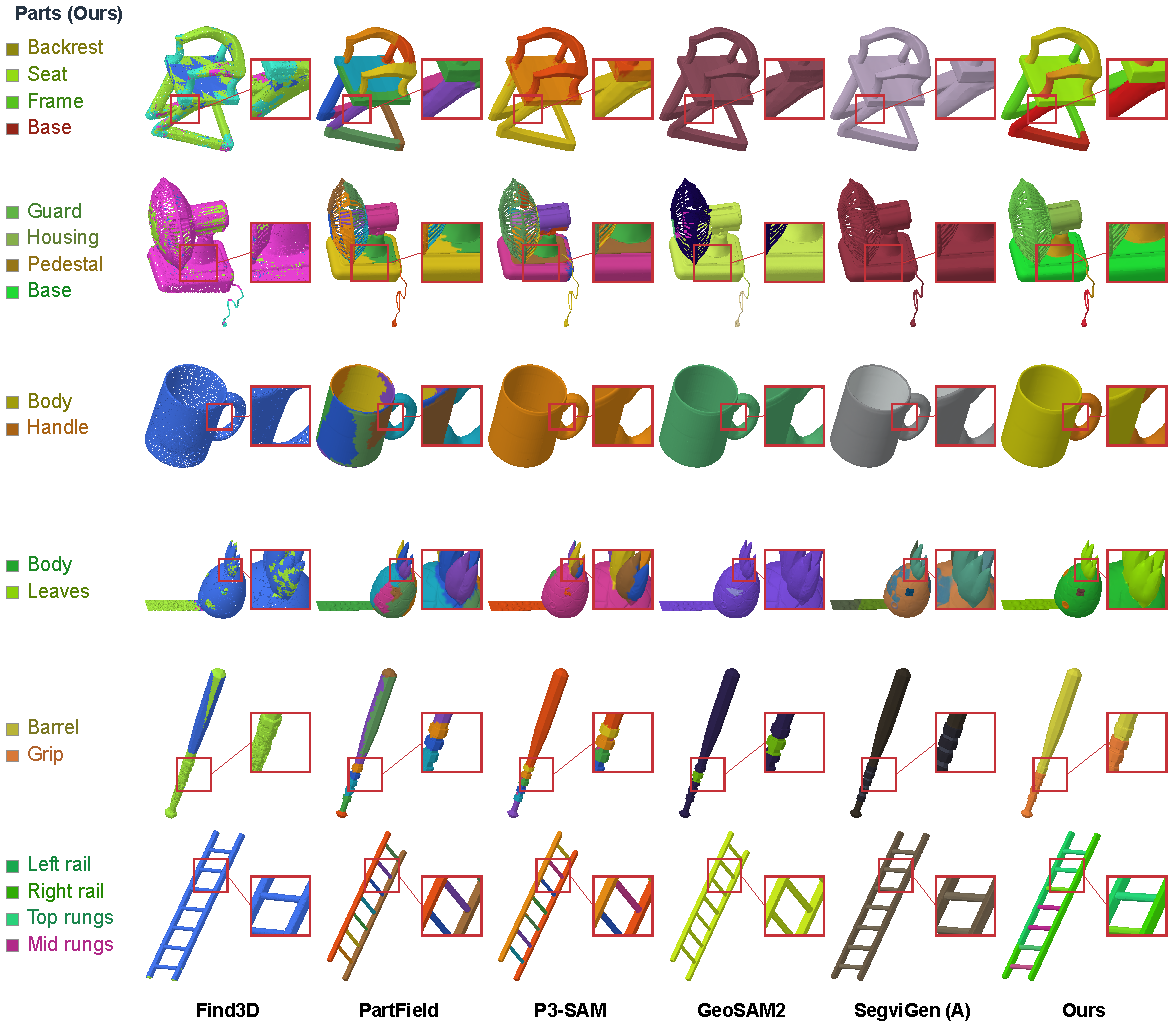
\includegraphics[width=\textwidth]{fig_sixmethod_3d_comparison_clean.pdf}
\caption{Six selected favorable cases with matched detail enlargements. Left labels name selected visible parts in Ours, and colors are local to each output. Rows share display views and scales. Find3D uses labeled points, and the other methods use meshes.}
\label{fig:sixmethod_qualitative}
\end{figure}

\subsection{Data and Evaluation Sets}
The Objaverse \citep{deitke2023objaverse} comparison uses 471 of the final 500 objects (146 assemblies, 179 solid-volume, and 146 thin or fine-grained). The other 29 include 24 unmerged records and five camera or protocol exclusions. Eight earlier objects fall outside the roster. The roster requires a completed C output, so the comparison describes the retained cohort.

The A/B/C/D and ablation runs share the same 471 unique identifiers (UIDs). Direct guidance analysis uses 440 B/C pairs and 479 C maps. Feedback and part-size analyses use an archived set of 500 objects (154/181/165). Records that are missing receive no score.

Our references use object-local IDs in place of a shared taxonomy \citep{lambert2023mseg}. All 500 reference maps were produced through model-assisted annotation. A model provided the initial mask draft for each object, one annotator manually corrected part boundaries and labels, and the corresponding author verified a sample of one map in five (20\%) before the maps entered scoring; maps outside the sample were retained as corrected. This check was performed by an author rather than by an independent annotator, and no automatic semantic validation was applied, so these scores measure agreement with the designated maps rather than validated ground truth. D receives the scoring map as guidance and measures reference-conditioned consistency. The separate mesh experiment in Section~\ref{sec:native_mesh} uses official annotations.

\begin{figure}[t]
\centering
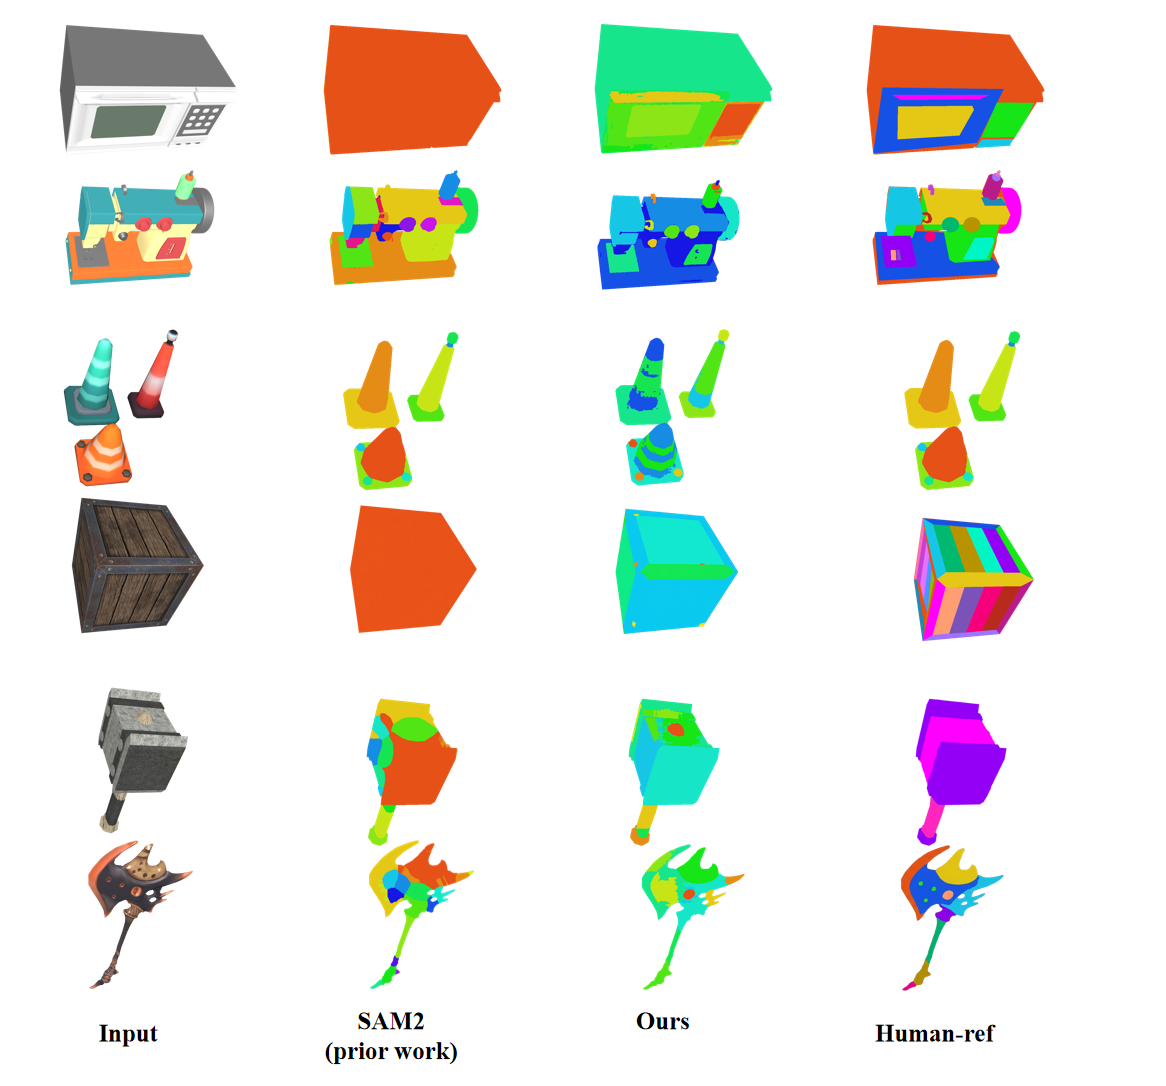
\includegraphics[width=0.92\textwidth]{fig3_guidance_clean.png}
\caption{Source images and guidance from automatic SAM2, Ours, and the designated reference. Row pairs show assemblies, solid-volume objects, and thin or fine-grained objects. Colors are local.}
\label{fig:guidance}
\end{figure}

\begin{table}[t]
\caption{Paired 2D guidance agreement (\%) on 440 objects after foreground alignment. Part F1 uses IoU 0.5, and differences use unrounded scores.}
\label{tab:guidance2d}
\centering
\setlength{\tabcolsep}{5pt}
\begin{tabular}{@{}lrrrr@{}}
\toprule
Guidance & mIoU & BF1@5px & BF1@2px & Part F1\\
\midrule
B (SAM2 \citep{ravi2024sam2}) & 45.86 & 50.44 & 45.74 & 40.84\\
C (Ours) & \textbf{52.88} & \textbf{54.38} & \textbf{47.55} & \textbf{44.07}\\
$\Delta$ (\%) & $+7.01$ & $+3.94$ & $+1.81$ & $+3.23$\\
\botrule
\end{tabular}
\end{table}

\begin{table}[t]
\caption{A/B/C/D projection agreement (\%) on the same 471 objects, geometry, settings, and cameras. Objects have equal weight, and D receives the scoring reference.}
\label{tab:controlled}
\setlength{\tabcolsep}{6pt}
\begin{tabular}{@{}lrrr@{}}
\toprule
Condition & mIoU & BF1@5px & Part F1\\
\midrule
A (Raw image) & 34.00 & 31.48 & 32.27\\
B (Automatic SAM2) & 35.78 & 32.66 & 40.79\\
C (Ours) & 38.14 & 35.88 & 36.84\\
D (Reference guidance) & 51.51 & 48.28 & 54.23\\
\botrule
\end{tabular}
\end{table}

\subsection{Implementation and Controlled Conditions}
Images and guidance are $1024\times1024$. Planning and audit use Qwen3-VL-4B-Instruct, and masks use SAM2.1 Hiera Base+ (\texttt{sam2.1\_hiera\_base\_plus.pt}). The palette, parser, orientation, and alpha threshold are fixed. The 500 C caches comprise 494 main-batch records and six from three recovery batches, with provenance retained.

SegviGen uses 512-resolution voxels, \texttt{full\_seg\_w\_2d\_map.ckpt}, 20 sampling steps, and seed 42. Export enables remeshing with a 100,000-face target and texture resolution 4096. Geometry and inference settings are shared per object, and manifests record input, configuration, and checkpoint identities.

\begin{figure}[t]
\centering
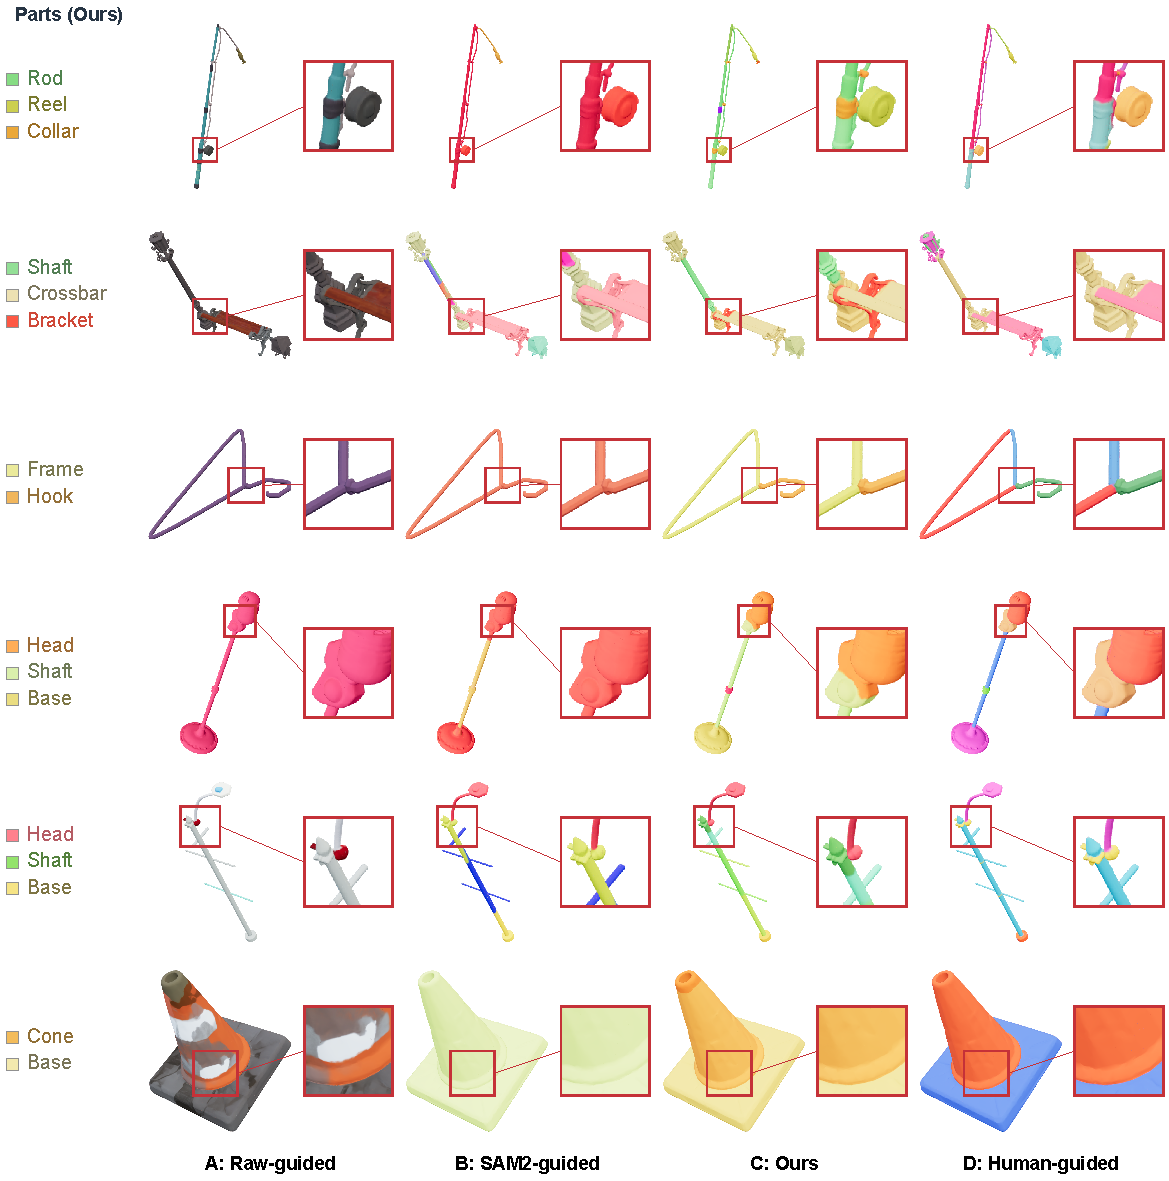
\includegraphics[width=\textwidth]{fig4_3d_comparison_clean.pdf}
\caption{Selected A/B/C/D outputs with matched detail enlargements and color-coded part names for Ours. Rows share display views, scales, and lighting, and scoring uses separate frozen cameras. Colors denote local regions.}
\label{fig:qualitative}
\end{figure}

\subsection{Comparison Methods}
We evaluate Find3D \citep{ma2024find3d}, PartField \citep{liu2025partfield}, P3-SAM \citep{ma2025p3sam}, GeoSAM2 \citep{deng2025geosam2}, and SegviGen \citep{li2026segvigen} under our protocol and report the results in Table~\ref{tab:main}. PartField uses $K=10$, seed 42, 32 face batches, and 1,000 samples per face. P3-SAM uses mesh cleaning, 100,000 points, 400 automatic prompts, batch size one, and seed 42. GeoSAM2 uses automatic views 0 and 6, 64 points per side and eight per batch, with shared guidance disabled. Settings remain fixed across objects. Find3D uses frozen Qwen3-VL queries from the raw image and D-repaired masks, and we report its 468-object group-macro mean separately because eight records lack queries.

\begin{table}[t]
\caption{Paired controls on 471 objects. Values are object-weighted percentages, with BF1@5px and Part F1 at IoU 0.5. Retry-box ordering fixes selected masks and initial points, and its output projection was not evaluated.}
\label{tab:ablation}
\setlength{\tabcolsep}{3pt}
\begin{tabular*}{\textwidth}{@{\extracolsep{\fill}}lrrrrrr@{}}
\toprule
 & \multicolumn{3}{c}{2D guidance} & \multicolumn{3}{c}{Output projection}\\
\cmidrule(lr){2-4}\cmidrule(l){5-7}
Configuration & mIoU & BF1 & Part F1 & mIoU & BF1 & Part F1\\
\midrule
Full & 53.92 & 55.54 & 44.92 & 38.11 & 35.85 & 36.69\\
Retry-box ordering & 54.08 & 55.82 & 44.95 & n/a & n/a & n/a\\
No mask audit & 54.18 & 55.74 & 45.48 & 38.35 & 36.09 & 36.33\\
No point filtering & 53.90 & 55.31 & 44.66 & 37.97 & 35.82 & 37.32\\
Large mask, no filter & 43.87 & 48.45 & 43.62 & 34.44 & 31.42 & 42.67\\
\botrule
\end{tabular*}
\end{table}

\subsection{Guidance and Projection Metrics}
We ignore labels $-1$ and $65535$. Background zero is excluded from the part list, but predicted spill into background remains in the union. For predicted regions $P_i$ and $n$ reference regions $D_j$, let $J_{ij}=|P_i\cap D_j|/|P_i\cup D_j|$. Since IDs differ across methods, matching evaluates partitions rather than names. Direct 2D frame alignment uses foreground silhouettes. Matched mIoU maximizes total overlap under a one-to-one partial assignment $\pi$ as
\begin{equation}
\operatorname{mIoU}_{\mathrm{match}}
=\frac1n\max_\pi\sum_{j\in\operatorname{dom}(\pi)}J_{\pi(j),j}.
\label{eq:matched}
\end{equation}
Unmatched reference parts contribute zero. Part F1 instead maximizes the number $T$ of pairs with IoU $\geq0.5$ and equals $2T/(m+n)$ for $m$ predictions.

BF1 complements region overlap \citep{cheng2021boundaryiou}. We sum boundary F1 over nonzero-overlap mIoU-matched pairs and divide by $n$, with zero for unmatched parts. Tolerances are two or five pixels at $1024\times1024$, using identical inputs within each cohort. Primary metrics weight the 471 objects (432 original, 39 extension) equally. Differences between two scores are absolute differences and are written in \%.

We project outputs to discrete labels with recorded cameras and transforms. The A/B/C/D and ablation runs require shared source identity, exact foreground and face-count preservation per arm, camera-to-source foreground IoU $\geq0.50$, and all six cross-arm foreground IoUs $\geq0.99$. Failure excludes the UID from every arm. External methods retain their recorded registration and camera gates, and scoring uses the original projections. Scores concern the visible partition, not volumetric IoU or unseen surfaces, and display views are separate.

\begin{table}[t]
\caption{Paired projection agreement (\%) by structure on the same 471 objects as in Table~\ref{tab:main}. Entries report mIoU / BF1@5px / Part F1@0.5, with object weighting within each group.}
\label{tab:projection_group}
\setlength{\tabcolsep}{3pt}
\begin{tabular*}{\textwidth}{@{\extracolsep{\fill}}lccc@{}}
\toprule
Method & \shortstack{Assemblies\\($N=146$)} & \shortstack{Solid volume\\($N=179$)} & \shortstack{Thin / fine-grained\\($N=146$)}\\
\midrule
P3-SAM \citep{ma2025p3sam} & 29.51 / 23.81 / 26.42 & 46.97 / 30.61 / 45.85 & 42.10 / 44.04 / 38.16\\
GeoSAM2 \citep{deng2025geosam2} & 12.70 / 8.91 / 16.18 & 40.69 / 28.14 / 51.99 & 21.54 / 20.74 / 31.59\\
PartField \citep{liu2025partfield} & 29.40 / 20.69 / 22.99 & 35.53 / 19.45 / 10.95 & 37.28 / 38.71 / 19.90\\
SegviGen (A) \citep{li2026segvigen} & 15.58 / 13.85 / 14.77 & 45.84 / 36.68 / 39.97 & 37.89 / 42.74 / 40.33\\
Ours & 24.57 / 21.74 / 25.16 & 46.36 / 38.32 / 42.43 & 41.61 / 47.02 / 41.65\\
\botrule
\end{tabular*}
\end{table}

\begin{table}[t]
\caption{Mask refinement on 500 archived objects with identical retained candidates and assembly anchors. Group-macro percentages use unrounded differences. Recall and Part F1 use IoU 0.5.}
\label{tab:audit}
\setlength{\tabcolsep}{8pt}
\begin{tabular}{@{}lccc@{}}
\toprule
Guidance & mIoU & Recall & Part F1\\
\midrule
Initial masks & 51.21 & 51.06 & 43.77\\
Selected masks & 51.53 & 51.70 & 43.72\\
\midrule
$\Delta$ (\%) & $+0.31$ & $+0.64$ & $-0.05$\\
\botrule
\end{tabular}
\end{table}

\begin{table}[t]
\caption{C guidance by structural group on 479 objects. Object-weighted percentages use BF1@5px and Part F1 at IoU 0.5.}
\label{tab:guidance_group}
\setlength{\tabcolsep}{8pt}
\begin{tabular}{@{}lrrrr@{}}
\toprule
Group & $N$ & mIoU & BF1 & Part F1\\
\midrule
Assemblies & 151 & 45.39 & 45.55 & 45.54\\
Solid volume & 179 & 56.18 & 55.56 & 37.58\\
Thin / fine-grained & 149 & 58.95 & 64.94 & 52.85\\
\botrule
\end{tabular}
\end{table}

\subsection{Comparison with Existing Methods}
In Table~\ref{tab:main}, Ours gains 4.14\% mIoU, 4.39\% BF1@5px, and 4.57\% Part F1 over raw-image SegviGen on 471 objects. Its BF1 leads all four paired baselines at both tolerances, whereas P3-SAM leads on mIoU and Part F1. Fig.~\ref{fig:summary}a summarizes these comparisons. In Fig.~\ref{fig:sixmethod_qualitative}, selected cases show the separation of the mug handle, bat grip, and fan support, alongside residual fragments.

\begin{figure}[t]
\centering
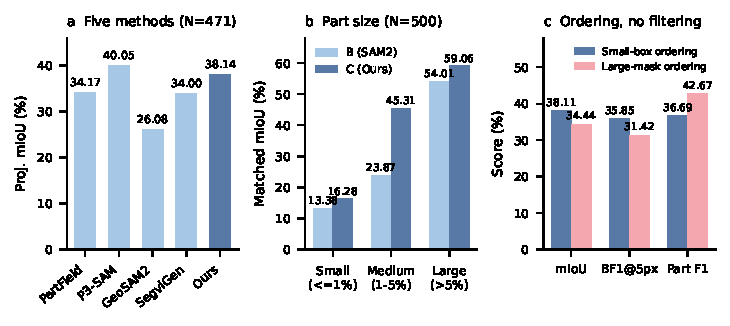
\includegraphics[width=\textwidth]{fig_summary_bars.pdf}
\caption{Summary of the main quantitative results. \textbf{a}, Projection agreement of five methods on 471 objects. \textbf{b}, Matched mIoU of B and C by part size on 500 archived objects. \textbf{c}, Projection agreement under small-box and large-mask ordering with point filtering disabled.}
\label{fig:summary}
\end{figure}

\subsection{Effect of Guidance on the Frozen Backend}
In Table~\ref{tab:guidance2d}, C gains 7.01\% mIoU and 3.23\% Part F1 in paired 2D guidance, with BF1 gains of 3.94\% and 1.81\% at five and two pixels. Its 479 available maps score 53.64\%, 55.32\%, and 44.84\% in mIoU, BF1@5px, and Part F1. In Fig.~\ref{fig:guidance}, B and D share the cone mask.

With geometry and inference fixed, Table~\ref{tab:controlled} shows that C gains 2.35\% mIoU and 3.21\% BF1 over B, with a 3.95\% lower Part F1. Reference guidance yields 51.51\% mIoU under D. In Fig.~\ref{fig:qualitative}, C separates the cone base and hanger hook, with a small extra region near the cone rim.

\subsection{Paired Mask and Assembly Controls}
Table~\ref{tab:ablation} reports controls on mask selection, filtering, and ordering with shared plans, candidates, initial masks, references, and cameras. No mask audit retains initial masks, and no point filtering bypasses both filters. Four configurations have backend outputs, reprojected together, and Full scores 38.11\%, compared with 38.14\% in the main run. Guidance scores decode RGB inputs, including palette reuse on four objects.

With point filtering disabled in both configurations, small-box ordering gains 10.02\% in 2D mIoU and 6.86\% in BF1 over decreasing mask-area ordering. Projection gains are 3.53\% and 4.40\%, while Part F1 falls by 5.34\%, as Fig.~\ref{fig:summary}c shows. Processing order affects the residual area available to each candidate and can determine whether it survives. This comparison measures the complete assembly rule, including its color assignment, rather than isolating original versus retry boxes.

Removing the audit raises projected mIoU and BF1 by 0.24\% each and lowers Part F1 by 0.36\%. Bypassing point filtering changes each projected mean by less than 0.7\%. Thus, the strongest measured assembly effect is the ordering trade-off, and the audit and point filtering yield smaller, metric-dependent changes.

The box control fixes selected masks and original points. Substituting valid retry boxes changes order on 101 of 471 objects and ownership on 75. Another 25 change RGB encoding alone, and one changes neither output. Comparing ownership by candidate ID excludes label renumbering. Retry boxes raise 2D mIoU by 0.17\% and BF1 by 0.28\%. This establishes sensitivity to box choice, without a measured advantage for the original boxes. The control has no backend outputs.

On 500 archived objects, mask replacement fixes the anchors and 3,546 of 4,627 candidates retained in production, and Table~\ref{tab:audit} reports the result. Selected masks reproduce production partitions and raise group-macro mIoU by 0.31\%. Among 283 objects with retries, 138 improve, 139 decline, and six tie.

\subsection{Structural Variation}\label{sec:structural_analysis}
In Table~\ref{tab:guidance_group}, C guidance scores highest on thin or fine-grained objects. In paired projections, Table~\ref{tab:projection_group} shows that Ours trails P3-SAM and PartField in assembly mIoU, and exceeds P3-SAM in BF1 by 7.71\% on solid objects and 2.98\% on thin objects.

\begin{table}[t]
\caption{Archived paired B/C structure analysis (\%). BF1 uses a 2px tolerance and recall uses IoU 0.5. $\Delta$ denotes C$-$B in \%. Group rows average objects, and other rows weight groups equally. $N$ denotes contributing objects, and n/a marks an undefined macro-average.}
\label{tab:strata}
\footnotesize
\setlength{\tabcolsep}{2pt}
\begin{tabular*}{\textwidth}{@{}l@{\hspace{3pt}}l@{\extracolsep{\fill}}rccccccccc@{}}
\toprule
Panel & Stratum & $N$ & \multicolumn{3}{c}{Matched mIoU} & \multicolumn{3}{c}{BF1@2px} & \multicolumn{3}{c}{Recall@0.5}\\
\cmidrule(lr){4-6}\cmidrule(lr){7-9}\cmidrule(l){10-12}
 & & & B & C & $\Delta$ & B & C & $\Delta$ & B & C & $\Delta$\\
\midrule
Group & Assemblies & 154 & 37.12 & 42.60 & $+5.48$ & 34.80 & 34.62 & $-0.19$ & 38.49 & 44.57 & $+6.08$\\
 & Solid volume & 181 & 50.50 & 56.35 & $+5.85$ & 49.42 & 49.23 & $-0.19$ & 51.15 & 52.15 & $+1.00$\\
 & Thin / fine-grained & 165 & 46.75 & 55.63 & $+8.88$ & 49.98 & 56.75 & $+6.76$ & 48.75 & 58.38 & $+9.63$\\
\midrule
Part count & 1 to 5 parts & 327 & 53.49 & 61.92 & $+8.43$ & 54.55 & 56.57 & $+2.01$ & 55.61 & 62.89 & $+7.28$\\
 & 6 to 10 parts & 107 & 34.91 & 44.47 & $+9.55$ & 31.90 & 37.81 & $+5.91$ & 35.15 & 46.63 & $+11.48$\\
 & $\geq$11 parts & 66 & n/a & n/a & n/a & n/a & n/a & n/a & n/a & n/a & n/a\\
\midrule
Part size & Small ($\leq$1\%) & 158 & 13.38 & 16.28 & $+2.90$ & 20.27 & 20.92 & $+0.65$ & 11.64 & 14.25 & $+2.61$\\
 & Medium ($>$1 to 5\%) & 261 & 23.87 & 45.31 & $+21.44$ & 32.50 & 45.19 & $+12.69$ & 22.12 & 47.20 & $+25.07$\\
 & Large ($>$5\%) & 500 & 54.01 & 59.06 & $+5.05$ & 49.98 & 50.73 & $+0.75$ & 56.42 & 59.54 & $+3.12$\\
\midrule
Overall & All objects & 500 & 44.79 & 51.53 & $+6.74$ & 44.74 & 46.87 & $+2.13$ & 46.13 & 51.70 & $+5.57$\\
\botrule
\end{tabular*}
\end{table}

The archived analysis in Table~\ref{tab:strata} bins parts by foreground-relative area after whole-object matching. C gains 6.74\% macro mIoU overall, with gains of 21.44\% on medium parts and 2.90\% on small parts, as Fig.~\ref{fig:summary}b shows. % TODO check: the text below reports the at-least-11-parts losses, but that row of the table is n/a. Add the per-group values to the table or reword.
With at least 11 parts, C loses 1.56\% on assemblies and 1.93\% on thin objects. The solid-volume bin is empty.

\subsection{Native Mesh Evaluation}\label{sec:native_mesh}
We prespecified 16 PartObjaverse-Tiny meshes by UID hash, two per category, disjoint from the main and development sets \citep{yang2024sampart3d}. A, B, and C share source meshes, views, and backend settings. We invert the export transform and assign each source face centroid its closest predicted surface label within two normalized voxel diagonals. Geometry review precedes reading official labels and requires 95\% assigned faces per arm. Unassigned faces remain in the metric. Official ground-truth-best (GT-best) IoU averages each reference part's best overlap, allowing predicted-region reuse, and then weights objects equally.

\begin{table}[t]
\caption{Official GT-best IoU (\%) on 14 paired meshes from 16 prespecified PartObjaverse-Tiny objects. Two C plans failed. Semantic and instance labels use the same geometry mapping.}
\label{tab:native_mesh}
\setlength{\tabcolsep}{8pt}
\begin{tabular}{@{}lrr@{}}
\toprule
Condition & Semantic & Instance\\
\midrule
A (Raw image) & 43.45 & 38.85\\
B (Automatic SAM2) & \textbf{45.24} & \textbf{46.93}\\
C (Ours) & 43.69 & 43.89\\
\botrule
\end{tabular}
\end{table}

Two C plans failed, leaving 14 paired meshes without replacement. In Table~\ref{tab:native_mesh}, C improves instance IoU over A on 10 meshes, averaging $+5.04$\%. Against B, it improves eight and declines on six, averaging $-3.04$\% instance and $-1.55$\% semantic IoU. Thus, the projection gain over B does not extend to these official mesh labels. This comparison tests the full pipeline, rather than anchor choice.

% Complete all experimental floats before the conclusion.
\FloatBarrier
\section{Conclusion}\label{sec:conclusion}
We separate revisable prediction prompts from the spatial anchors used to assemble a conditioning partition. Fixed-mask controls show that assembly boxes affect pixel ownership independently of mask prediction. On 471 objects, small-box ordering improves projected overlap and boundaries relative to large-mask ordering, at a cost in Part F1. The full guidance pipeline improves projection agreement over raw-image SegviGen, while automatic SAM2 leads on the paired native meshes. These findings distinguish the effect of assembly from the quality of the masks it receives.

\section*{Acknowledgements}
We thank Changjian Yu of Lanzhou University Wales College for manually correcting the model-drafted reference annotations used in this study.

\section*{Declarations}

\textbf{Funding.} The authors acknowledge the National Natural Science Foundation of China (Grants 62606208 and 62606209), the Supercomputing Center of Lanzhou University, and the Talent Scientific Fund of Lanzhou University for their support.

\textbf{Competing interests.} The authors declare no competing interests.

\textbf{Ethics approval.} Public-data research required no ethics approval.

\textbf{Data availability.} Manifests, reference annotations, and per-object scores are available from the corresponding authors on reasonable request, subject to source-asset licenses. All reference annotations were model-drafted and manually corrected before release.

\textbf{Code availability.} The code is available at \codeurl.

\textbf{Author contributions.} Yulin Fu led conception, method development, experiments, and writing. Cheng Yang and Qing Ai assisted comparisons, validation, and settings checks, and Qibin Hu contributed discussions and feasibility analysis. Jisheng Dang, Bin Hu, Wei-Shi Zheng, Qi Tian, and Tat-Seng Chua supervised, coordinated, and revised the work. All authors approved the manuscript.

\textbf{Use of AI tools.} Codex and Gemini assisted experimental-design review and language editing. Codex also inspected geometry overlays before native scoring. In addition, the reference annotations were initialized by a model and manually corrected by annotators, as described in the Data and Evaluation Sets section. The authors retain responsibility for the manuscript and results.

\bibliography{references}

\end{document}
